% This file provides an example Beamer presentation using the RWTH theme
% showcasing some of the more common options, similar to the Powerpoint version
% 12.11.2014: Revision 1 (Harold Bruintjes, Tim Lange)

% For RWTH, beamer should be loaded with class option t (top)
\documentclass[t]{beamer}

% Use fontspec to get Arial font
% Requires use of XeLaTeX
\usepackage{fontspec}
\setmainfont{Arial}
\setsansfont{Arial}
% Also force Arial for math for a more consistent look
\usepackage{unicode-math}

\usepackage[utf8]{inputenc}
\usepackage[ngerman]{babel}
\usepackage{csquotes}
\usepackage{hyperref}
\usepackage{xcolor}
\definecolor{rwthblue}{RGB}{0, 84, 159}
% www.colorhexa.com for color references

% ---------- Hyperref -----------
\hypersetup{colorlinks=true,
            breaklinks=true,
            urlcolor=rwthblue,
            linkcolor=rwthblue,
            citecolor=rwthblue}
\def\UrlBreaks{\do\/\do-}
% -------------------------------

% https://tex.stackexchange.com/questions/426088/texlive-pretest-2018-beamer-and-subfig-collide
\makeatletter
\let\@@magyar@captionfix\relax
\makeatother

% German style date formatting (footer)
\usepackage[ddmmyyyy]{datetime}
\renewcommand{\dateseparator}{.}

\usepackage{MnSymbol,wasysym}

% Format the captions used for figures etc.
\usepackage[compatibility=false]{caption}
\captionsetup{singlelinecheck=off,justification=raggedleft,labelformat=empty,labelsep=none}

% PGFPlots is used for drawing some of the charts
\usepackage{pgfplots}
\pgfplotsset{compat=newest}
% This file contains some styles and macros for drawing charts similar to those of MS Office

\pgfplotsset{hor_barchart/.style={
  xbar=0mm,
  xmin=0,
  xtick=\empty,
  axis y line*=left,
  x axis line style={opacity=0},
  bar width=0.6cm,
  ytick=data,
  nodes near coords,
  every axis/.append style={font=\normalsize},
  every node near coord/.append style={font=\normalsize},
  nodes near coords align={horizontal},
  legend style={at={(0,-10mm)},anchor=north west,legend columns=-1,draw=none},
}}

\pgfplotsset{ver_barchart/.style={
  ybar=0mm,
  x = 4.5cm,
  ymin=0,
  ymajorgrids,
  axis x line*=bottom,
  y axis line style={opacity=0},
  bar width=0.8cm,
  enlarge x limits={0.15},
  xtick=data,
  nodes near coords,
  every axis/.append style={font=\normalsize},
  every node near coord/.append style={font=\normalsize},
  nodes near coords align={vertical},
  legend style={at={(0,-10mm)},anchor=north west,legend columns=-1,draw=none},
}}

\tikzstyle{chart}=[
    legend label/.style={font={\normalsize},anchor=west,align=left},
    legend box/.style={rectangle, draw=none, minimum size=5pt},
]

\tikzstyle{pie chart}=[
    chart,
    slice/.style={line cap=round, line join=round,draw=none},
    pie title/.style={font={\bf}},
    slice type/.style 2 args={
        ##1/.style={fill=##2},
        values of ##1/.style={}
    }
]

\newcommand{\pie}[3][]{
    \begin{scope}[#1]
    \pgfmathsetmacro{\curA}{90}
    \pgfmathsetmacro{\r}{1}
    \def\c{(0,0)}
    \node[pie title] at (90:1.3) {#2};
    \foreach \v/\s in{#3}{
        \pgfmathsetmacro{\deltaA}{\v/100*360}
        \pgfmathsetmacro{\nextA}{\curA + \deltaA}
        \pgfmathsetmacro{\midA}{(\curA+\nextA)/2}

        \path[slice,\s] \c
            -- +(\curA:\r)
            arc (\curA:\nextA:\r)
            -- cycle;

        %\begin{pgfonlayer}{foreground}
        % Position labels at 1.2 times radius (just outside of chart)
        \path \c -- node[pos=1.2,pie values,values of \s]{$\v\%$} +(\midA:\r);
        %\end{pgfonlayer}

        \global\let\curA\nextA
    }
    \end{scope}
}

% Custom legend (used for pie chart)
\newcommand{\legend}[2][]{
\begin{scope}[#1]
  \path
    \foreach \n/\s in {#2} {
      ++(0,-5pt) node[\s,legend box] {} +(5pt,0) node[legend label] {\n}
    };
\end{scope}
}


% Load the actual RWTH theme. Suggested is to load the full theme,
% as it requires some specific dimensions
\usetheme{rwth}

\begin{document}

\logo{
\includegraphics{logo.png}}

% Setup presentation information
\title{Back-Propagation and Algorithms for Training Artificial Neural Networks with TensorFlow}
\date{5. Februar 2021}
\author{Gero Kauerauf}

\frame{\titlepage}

\section{Deep Learning}

% Frame with items
\begin{frame}
\begin{itemize}
    \item Was kann \emph{Deep Learning}, was herkömmliche Algorithmen nicht können?
    \begin{itemize}
        \item Viele Probleme die Menschen intuitiv lösen sind mathematisch schwer zu beschreiben \\
        Keine präzise mathematische Beschreibung \(\rightarrow\) Kein Lösungsalgorithmus
        \item Deep Learning \emph{Modelle} sind in der Lage, solche Probleme zu lösen \newline
        \item Bsp.: Bilderkennung \\
        \enquote{Wie erkennt man eine Katze?}
    \end{itemize}
\end{itemize}
\begin{figure}
    \centering
    \begin{minipage}{0.5\textwidth}
        \centering
        \includegraphics[width=0.5\textwidth]{./images/paula.jpg} % first figure itself
    \end{minipage}\hfill
    \begin{minipage}{0.5\textwidth}
        \centering
        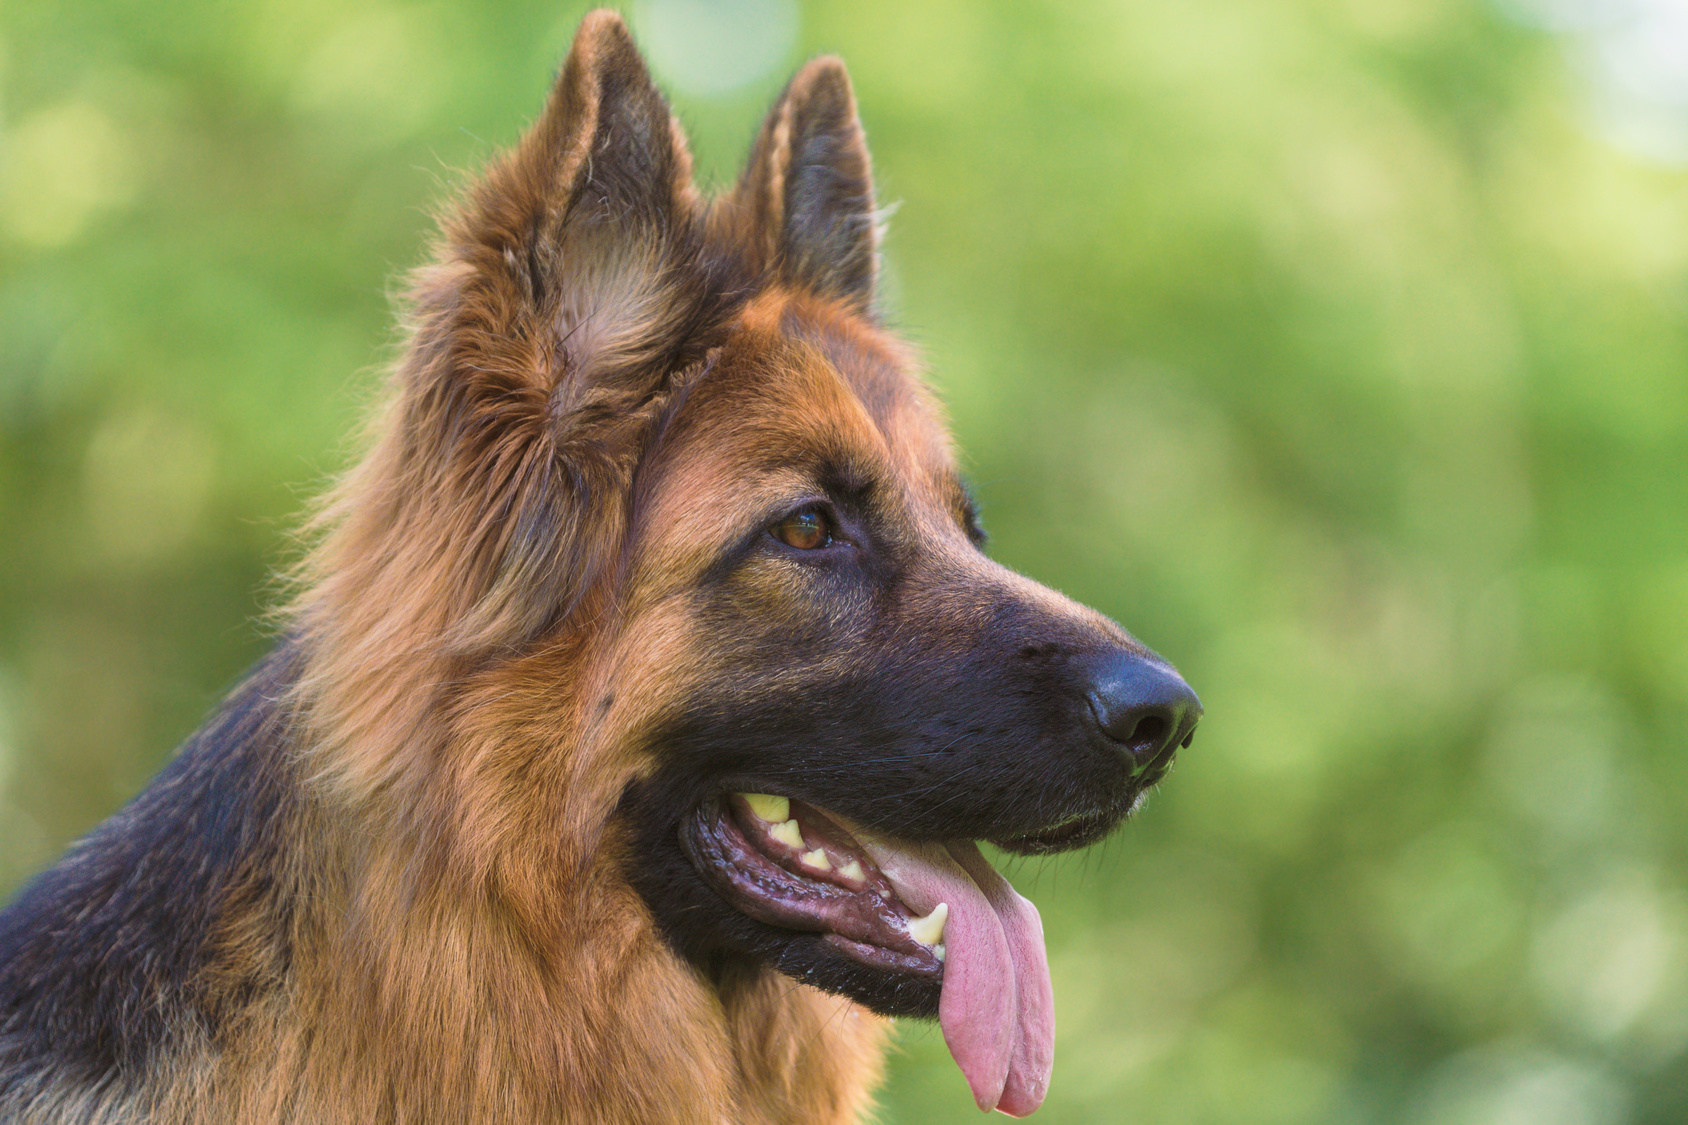
\includegraphics[width=0.9\textwidth]{./images/deutscher-schaeferhund.jpg} % second figure itself
    \end{minipage}
\end{figure}
\end{frame}

\section{Deep Learning}
\begin{frame}
    \begin{itemize}
        \item Ein weiteres Beispiel sind \emph{Spiele}, bei denen es \emph{praktisch} nicht möglich ist eine \emph{Gewinnstrategie} zu berechnen
        \begin{itemize}
            \item Beim Schach beläuft sich die Anzahl der möglichen Spielverläufe nach schon \(40\)-Zügen auf \(10^{115} - 10^{120}\)
            \newline
        \end{itemize}
        \item[\(\rightarrow\)] Ist eine mathematische Beschreibung schwer, oder ein Problem zu komplex, so können \emph{Deep Learning Modelle} helfen
    \end{itemize}
\end{frame}

\section{Inhalt des reports}
\begin{frame}
    \begin{itemize}
        \item Zentrale Frage: \newline 
        \begin{itemize}
            \item \enquote{\emph{Wie trainiert man ein neuronales Netz?}} \newline
        \end{itemize}
        \item Erläuterung der einzelnen Schritte beim Training eines neuronalen Netzes \newline
        \item Inhalt: \newline
        \begin{itemize}
            \item Feedforward networks
            \item Computational graphs \& Cost functions
            \item Back-Propagation \(\leftarrow\) \emph{algorithmisches Differenzieren}
            \item Stochastic Gradient Descent \(\leftarrow\) \emph{iteratives Lösungsverfahren}
        \end{itemize}

    \end{itemize}
\end{frame}

\section{Feedforward Network}
\begin{frame}
    \begin{itemize}
        \item Neural Network:
    \end{itemize}
    \begin{figure}
        \centering
        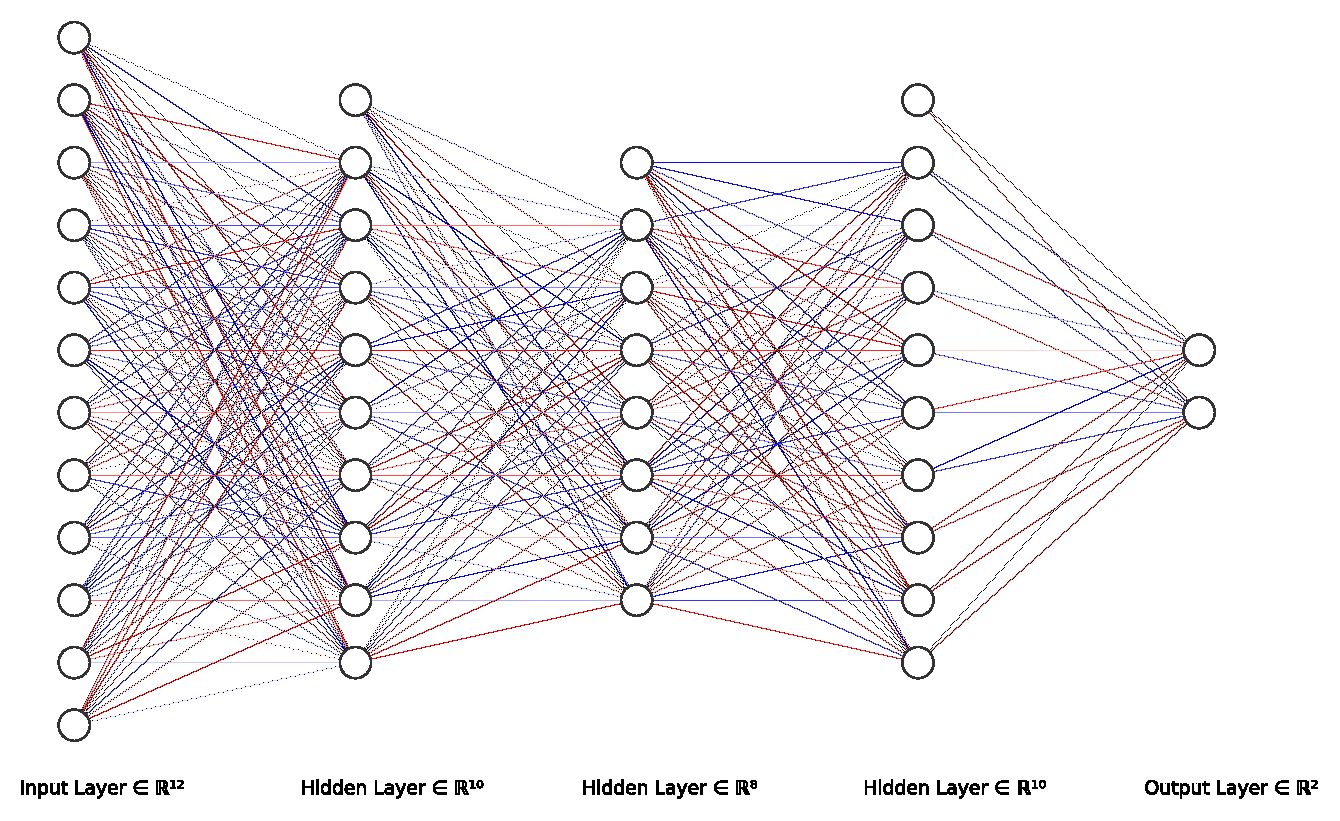
\includegraphics[width=0.8\textwidth]{./images/example-nn-crop.pdf}
    \end{figure}
\end{frame}

\section{Kostenfunktion}
\begin{frame}
    \begin{itemize}
        \item Für ein neuronales Netz kann man dann eine Kostenfunktion aufstellen
        \item Diese beschreibt den Fehler, um den sich die Ausgabe des neuronalen Netzes vom tatsächlichen Wert unterscheidet \newline
        \item Bsp.: Kleinste-Quadrate Methode \newline
        \item[\(\rightarrow\)] Minimiert man den Fehler und passt die Gewichte dementsprechend an, so verbessert man das Netz \newline
        \item Um ein Minimum zu finden brauchen wir die Ableitung
    \end{itemize}
\end{frame}

\section{Computational Graphs}
\begin{frame}
    \begin{figure}
        \centering
        \begin{minipage}{0.45\textwidth}
            \begin{figure}[]
                \centering
                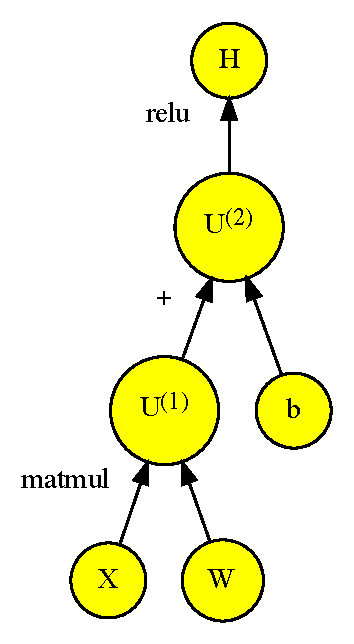
\includegraphics[width=0.7\textwidth]{../plots/computational-graph-c-crop.pdf}
            \end{figure}
        \end{minipage}\hfill
        \begin{minipage}{0.45\textwidth}
            \begin{itemize}
                \item Zuerst berechnen wir \(XW\) und speichern das Ergebnis in \(U^{(1)}\)
                \item Danach berechnen wir \(U^{(2)} = U^{(1)} + b \; \Leftrightarrow \; U^{(2)} = XW + b\)
                \item ReLU steht für \emph{rectifier linear unit}
                \item \(\rightarrow f(x) = \max\{0, x\}\) \newline
                \item Das bedeutet, dass dieser \enquote{computational graph} \(H = \max\{0, XW + b\}\) beschreibt
            \end{itemize}
        \end{minipage}
        \caption{\href{http://www.deeplearningbook.org}{www.DeepLearningBook.org}}
    \end{figure}
\end{frame}

\section{Back-Propagation}
\begin{frame}
    \begin{itemize}
        \item Back-Propagation ist \enquote{Graph-Algorithmus} der den Gradienten eines solchen Graphen bestimmen kann
        \item Dabei nutzt Back-Propagation \emph{rekursiv} die \emph{Kettenregel} \newline
        \item Bei der Back-Propagation handelt es sich somit um \enquote{algorithmisches Differenzieren}
    \end{itemize}
\end{frame}

\begin{frame}
    \begin{figure}
        \centering
        \begin{minipage}{0.45\textwidth}
            \begin{figure}[]
                \centering
                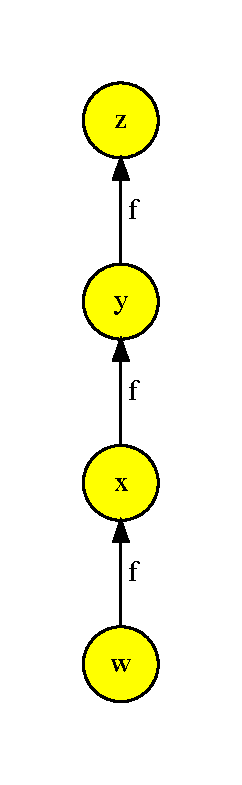
\includegraphics[width=0.4\textwidth]{./images/back-prop.pdf}
            \end{figure}
        \end{minipage}\hfill
        \begin{minipage}{0.45\textwidth}
            \begin{itemize}
                \item \(x = f(w)\), \(y = f(x)\), \(z = f(y)\)
                \item Wir wollen nun \(\frac{\partial z}{\partial w}\) berechnen
            \end{itemize}
            \begin{align*}
                \frac{\partial z}{\partial w} &= \frac{\partial z}{\partial y} \frac{\partial y}{\partial x} \frac{\partial x}{\partial w} \\
                &= f\prime(y) f\prime(x) f\prime(w) \\
                &= f\prime(f(f(w)))f\prime(f(w))f\prime(w)
            \end{align*}
        \end{minipage}
        \caption{\href{http://www.deeplearningbook.org}{www.DeepLearningBook.org}}
    \end{figure}
\end{frame}

\section{Gradientenverfahren}
\begin{frame}
    \begin{itemize}
        \item Das Gradientenabstiegsverfahren ist ein iterativer Algorithmus, zum lösen von Optimierungsproblemen \newline
        \item Im \enquote{Machine Learning} wird allerdings eine stochastische Abwandlung, das \emph{stochastische Gradientenverfahren} (SGD) genutzt \newline
        \item In Modulen wie TensorFlow basieren viele \enquote{Optimierer} auf SGD \newline
        \item[\(\rightarrow\)] SGD ist bei Kostenfunktionen so gut, da diese meistens eine Summe sind
    \end{itemize}
\end{frame}

\begin{frame}
    \begin{itemize}
        \item Beispielfunktion:
    \end{itemize}
    \begin{figure}
        \centering
        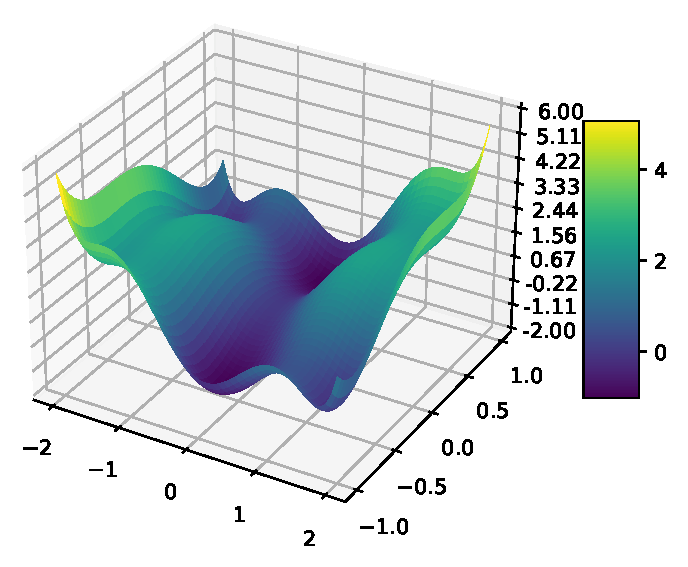
\includegraphics[width=0.65\textwidth]{./images/six-hump-camel-function-crop.pdf}
    \end{figure}
\end{frame}

\section{Interesse?}
\begin{frame}
    \begin{itemize}
        \item In meinem \emph{Report} gebe ich einen ersten Einblick in das Thema \emph{Deep Learning} \newline
        \item Die erwähnten Schritte beim Training eines \emph{Feedforward Networks} sind ausführlich erklärt \newline
        \item Auch die \emph{lineare Algbra} die hinter einem Netzwerk steckt wird beschrieben
    \end{itemize}
\end{frame}

\section{Quellen}
\begin{frame}
    \begin{itemize}
        \item Sources:
        \begin{itemize}
            \item \textbf{Deep Learning} by Ian Goodfellow and Yoshua Bengio and Aaron Courville \newline
            \href{https://www.deeplearningbook.org}{www.deeplearningbook.org}
            \item \textbf{TensorFlow} \newline
            \href{https://www.tensorflow.org}{www.tensorflow.org}
            \item \textbf{SFU} Virtual Library of Simulation Experiments: Test Functions and Datasets \newline
            \href{http://www.sfu.ca/~ssurjano/camel6.html}{http://www.sfu.ca}
            \item And of course wikipedia for quick look ups \newline
        \end{itemize}
        \item Tools used:
        \begin{itemize}
            \item \textbf{NN-SVG} \newline
            \href{http://alexlenail.me/NN-SVG/index.html}{http://alexlenail.me}
            \item \textbf{Graphviz} \newline
            \href{https://graphviz.org}{www.graphviz.org}
            \item \textbf{matplotlib} for more plots \newline
            \href{https://matplotlib.org}{www.matplotlib.org}
        \end{itemize}
    \end{itemize}
\end{frame}

\end{document}
